\documentclass{article}
\usepackage[margin=3cm]{geometry}
\usepackage[utf8]{inputenc}
\usepackage{amsmath}
\usepackage{amssymb}
\usepackage{float}
\usepackage{enumitem}
\usepackage{graphicx}
\usepackage{caption}
\usepackage{subcaption}

\graphicspath{ {Plots/} }

\begin{document}
	\textit{MS-E2134 - Decision making and problem solving}
	\vfill
	{\centering \Huge Assignment 2 \par}
	\vfill
	Christian Segercrantz - 481056 \\
	\par \today
	\pagebreak
	\tableofcontents
	\pagebreak
\section{Simulation}
\subsection{a)}
\begin{figure}[H]
	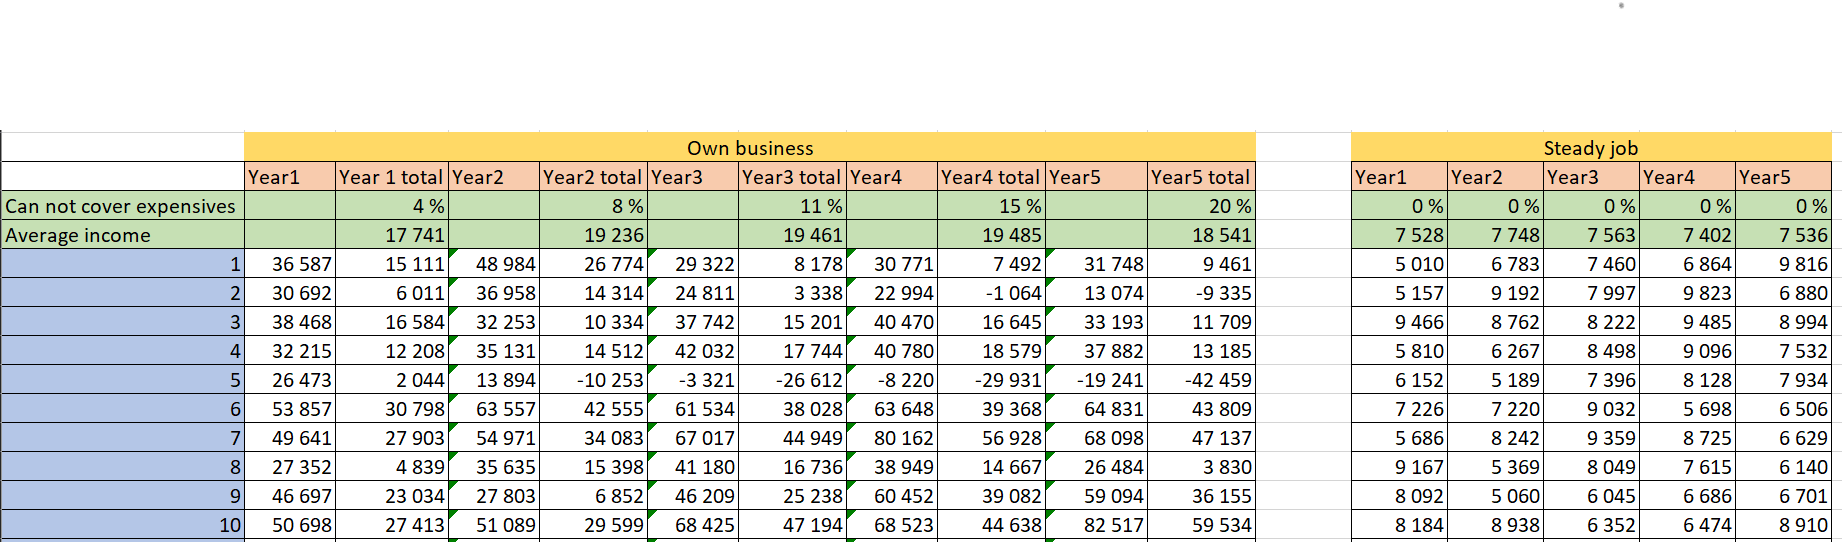
\includegraphics[width=\textwidth]{1a.png}
	\caption{Capion here}
	\label{fig:1a}
\end{figure}

\subsection{b)}

	\begin{table}[h]
		\centering
		\caption{Average cash flow for fives years for both the steady job and own business ventures.}
		\label{tab:1b}
		\begin{tabular}{l|l|l|l|l|l|}
			\cline{2-6}
			& Year 1 & Year 2 & Year 3 & Year 4 & Year 5 \\ \hline
			\multicolumn{1}{|l|}{Steady job}   & 7 528  & 7 748  & 7 563  & 7 402  & 7 536  \\ \hline
			\multicolumn{1}{|l|}{Own business} & 17 741 & 19 236 & 19 461 & 19 485 & 18 541 \\ \hline
		\end{tabular}
	\end{table}
	
	Based on the simulations, it seems that starting a own business venture would for sure be the more lucrative, and better, option. However, an average over 200 replications might give us an overly optimistic outlook.
\subsection{c)}
	We can see the probabilities from Table \ref{tab:1c}. We can see that initially the probability is approximately 5\% and rises to approximately 20\% in year 5. For the steady job, as the maximum of the expenses is less than the constant income, the probability that he is not able to cover his expenses is 0\% for all years.
	\begin{table}[h]
		\centering
		\caption{Probability that Dr. Cuckoo cannot cover his expenses each year for both the steady job and own business ventures.}
		\label{tab:1c}
		\begin{tabular}{l|l|l|l|l|l|}
			\cline{2-6}
			& Year 1 & Year 2 & Year 3 & Year 4 & Year 5 \\ \hline
			\multicolumn{1}{|l|}{Steady job}   & 0 \%   & 0 \%   & 0 \%   & 0 \%   & 0 \%   \\ \hline
			\multicolumn{1}{|l|}{Own business} & 4 \%   & 8 \%   & 11 \%  & 15 \%  & 20 \%  \\ \hline
		\end{tabular}
	\end{table}
\section{Decision trees}
\section{Elicitation of utility functions}
	We start by calculating the different values for the utility functions. We normalize the utility function such that $u(10M)=1$ and $u(-2M)=0$. We can thus calculate:
	\begin{align}
		u(1.5\text{M}) &= 0.5u(10\text{M}) + 0.5u(-2\text{M})\\
		u(1.5\text{M}) &= 0.5 \cdot 1 + 0.5 \cdot 0 \\ 
		u(1.5\text{M})&= 0.5 \\
		u(4\text{M}) &= 0.5u(10\text{M}) + 0.5u(1.5\text{M})\\
		u(4\text{M}) &= 0.5 \cdot 1 + 0.5 \cdot 0.5 \\ 
		u(4\text{M})&= 0.75 \\
		u(0.1\text{M}) &= 0.5u(-2\text{M}) + 0.5u(1.5\text{M})\\
		u(0.1\text{M}) &= 0.5 \cdot 0 + 0.5 \cdot 0.5 \\ 
		u(0.1\text{M})&= 0.25 \\
		u(6\text{M}) &= 0.4u(10\text{M}) + 0.6u(4\text{M})\\
		u(6\text{M}) &= 0.4 \cdot 1 + 0.6 \cdot 0.75\\ 
		u(6\text{M})&= 0.85 \\
	\end{align}
	The plotted utility function can be seen in Figure \ref{fig:3}. As we can see, the function is somewhat concave. According to EUT, Dr. Stoveo is, as he says, risk averse.
	\begin{figure}[H]
		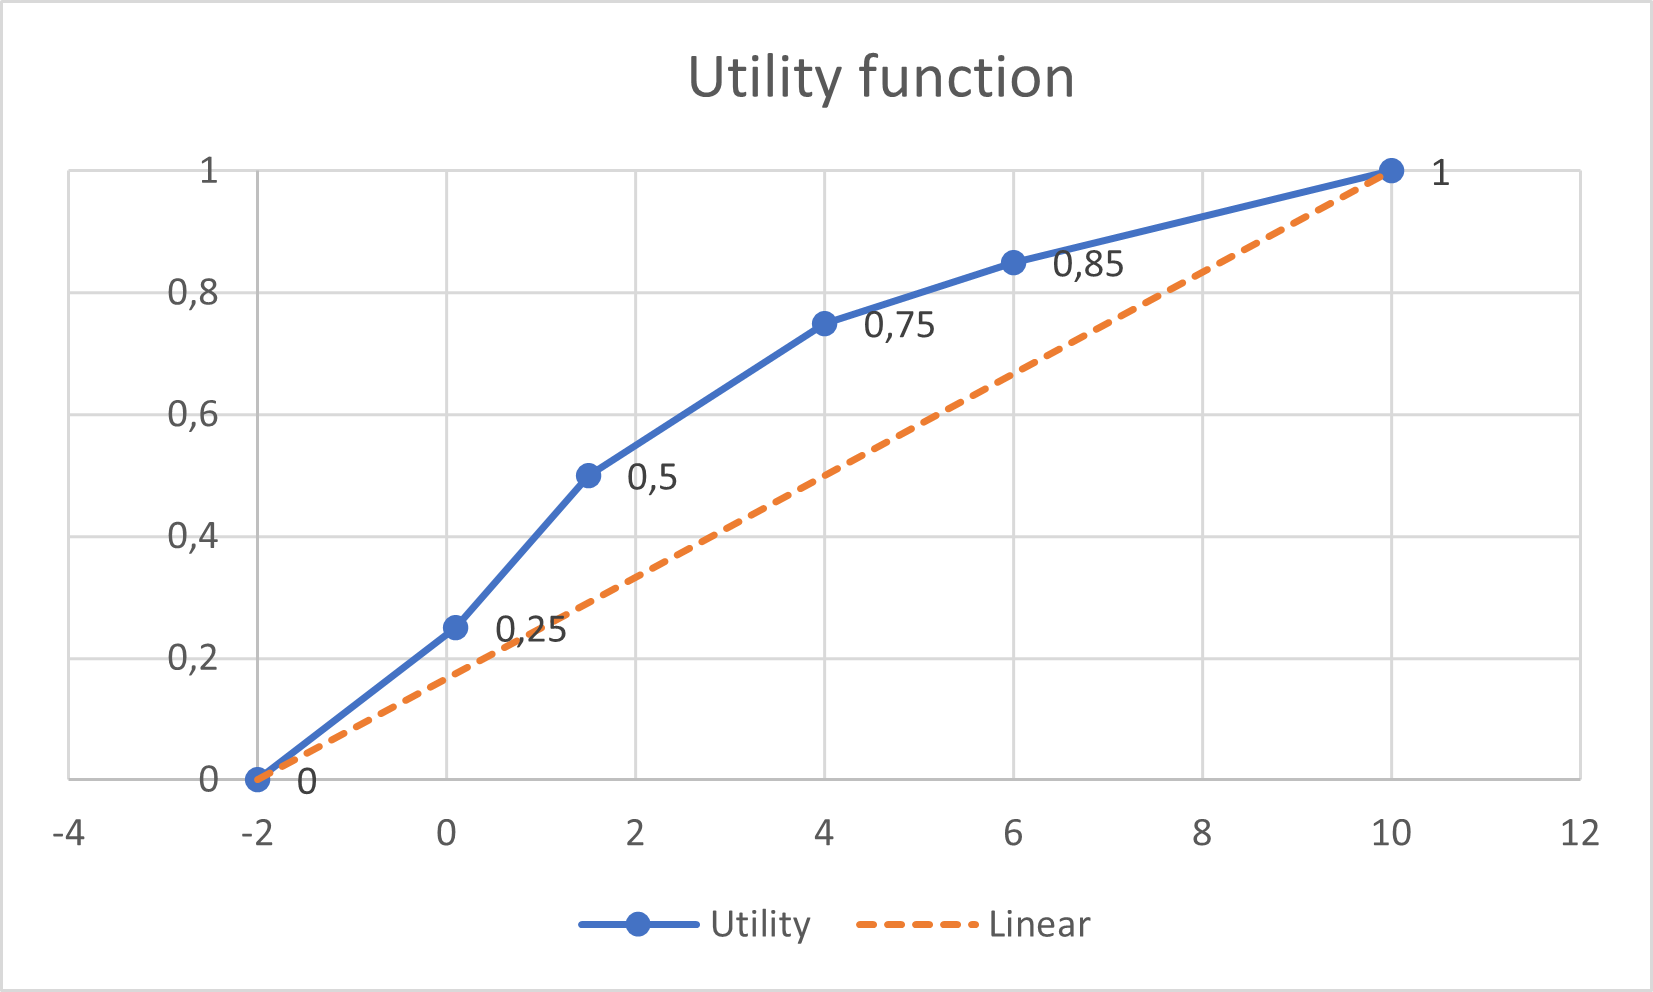
\includegraphics[width=0.9\textwidth]{3.png}
		\caption{The plotted utility function based on Dr. Stoveos choices.}
		\label{fig:3}
	\end{figure}
\section{Expected utility, risk-attitude, and risk measures}
\subsection{a)}
	In order to find out what the investors risk attitude is, we will use first and second order derivaties. 
	\begin{align}
		\frac{d}{dx}\sqrt{x} &= \frac{1}{2}x^{-\frac{1}{2}} \\
		\frac{d^2}{dx^2}\sqrt{x} &= -\frac{1}{4}x^{-\frac{3}{2}} \\
		\frac{d}{dx}x^3 &=  3x^2\\
		\frac{d^2}{dx^2}x^3 &= 6x
	\end{align}
	From these we can see that Rick Averell's utility functions first order derivative is always positive and hence is the utility function increasing. The second order derivative is always negative the growth is decreasing. From this we can conclude that the function is concave and Rick Averell is risk averse.
	We can draw conclusions in the same way for Ricki Seeck. Since both order derivatives are positive, we know that the function is increasingly positive and thus convex. Mr. Seeck's utility function is thus risk seeking. 
\subsection{b)}
\subsubsection{i}
	We can calculate the expected utility as $E[u(X)] = \int f_x(x) u(x)dx$. 
	\begin{equation}
		f_x(t) = 
		\begin{cases}
			 \frac{1}{50}, &  50 \leq x \leq 100 \\
			 0, & \mbox{otherwise}
		\end{cases}
	\end{equation}
	By integrating over the whole space we get,:
	\begin{align}
		\int f_x(x) u(x)dt &= \\
		\int_{50}^{100} \frac{1}{50} u(x) dt& 
	\end{align}
	We count the expected utility for Rick Averell:
	\begin{align}
		\int_{50}^{100} \frac{1}{50} \sqrt{x} dx &=  \\
		\Bigg/_{50}^{100} \frac{1}{50} \frac{3}{2} x^{\frac{3}{2}} = \frac{3}{2} x^{\frac{3}{2}} &= \\
		\Bigg/_{50}^{100} \frac{3}{100} x^{\frac{3}{2}}	& \approx 8.62		
	\end{align}
	Using the same logic we calculate the expected utility for Ricki Seeck:
	\begin{equation}
		\int_{50}^{100} \frac{1}{50} x^3 dx  = 468750.	
	\end{equation}
	To summarize, the expected utilities are $E[u(X)]_{Rick Averall} \approx 8.62$ and $E[u(X)]_{Ricki Seeck} = 468750$
	
	The certainty equivalent is calculated by $CE[x] = u^{-1}(E[u(X)])$. For Rick Averall this means
	\begin{equation}
		CE[x]_{Rick Averall} = u^{-1}(E[u(X)]) = E[u(X)]_{Rick Averall}^2 \approx 74.3
	\end{equation}
	and for Ricki Seeck 
		\begin{equation}
		CE[x]_{Ricki Seeck} = u^{-1}(E[u(X)]) = \sqrt[3]{E[u(X)]_{Ricki Seeck}} \approx 77.7.
	\end{equation}

	The risk premia is calculated as $RP[X] = E[X] - CE[X]$. 
	For Rick Averall this becomes:
	\begin{equation}
		E[u(X)]_{Rick Averall} - CE[x]_{Rick Averall} \approx -65.7,
	\end{equation}
	and for Ricki Seeck:
		\begin{equation}
		E[u(X)]_{Ricki Seeck} - CE[x]_{Ricki Seeck} \approx 468 672
	\end{equation}
	%Seems not to be in line with the attidude???
\end{document}